\chapter{Management Summary}


\subsubsection{Context}

A major challenge of writing software has always been to keep created source code maintainable. Early in the history of software development, modules have been used to structure code in manageable pieces and to make it reusable. With the rise of distributed systems, engineers started to implement services communicating with each other over a network. Coupling between such services has gained relevance as aspects like consistency or release cycles have become more challenging.

Several methodologies exist to guide a software architect when he or she designs services. \enquote{Service Oriented Architecture} is especially common in enterprise environments, microservices became popular in recent years. Leaving technical differences aside, all approaches share a common challenge: How can a big collection of data and functionality be decomposed into smaller pieces while retaining high cohesion and low coupling.

\subsubsection{A Structured Approach to Service Decomposition}

We found no extensive description of architecturally significant requirements in existing literature on distributed systems that optimize loose coupling and high cohesion in service decomposition. We therefore compiled a catalog of 16 \glspl{couplingCriterion} that aims to form a comprehensive but not conclusive collection based on literature and the input of our industry partner and our advisor. 

These coupling criteria help a software architect to structure architecturally significant requirements influencing the service decomposition decisions. Figure \ref{fig:cc-catalog-mgmt-summary} outlines the criteria catalog structured in viewpoints (rows) and criteria types (columns).
 
\begin{figure}[H]
	\centerline{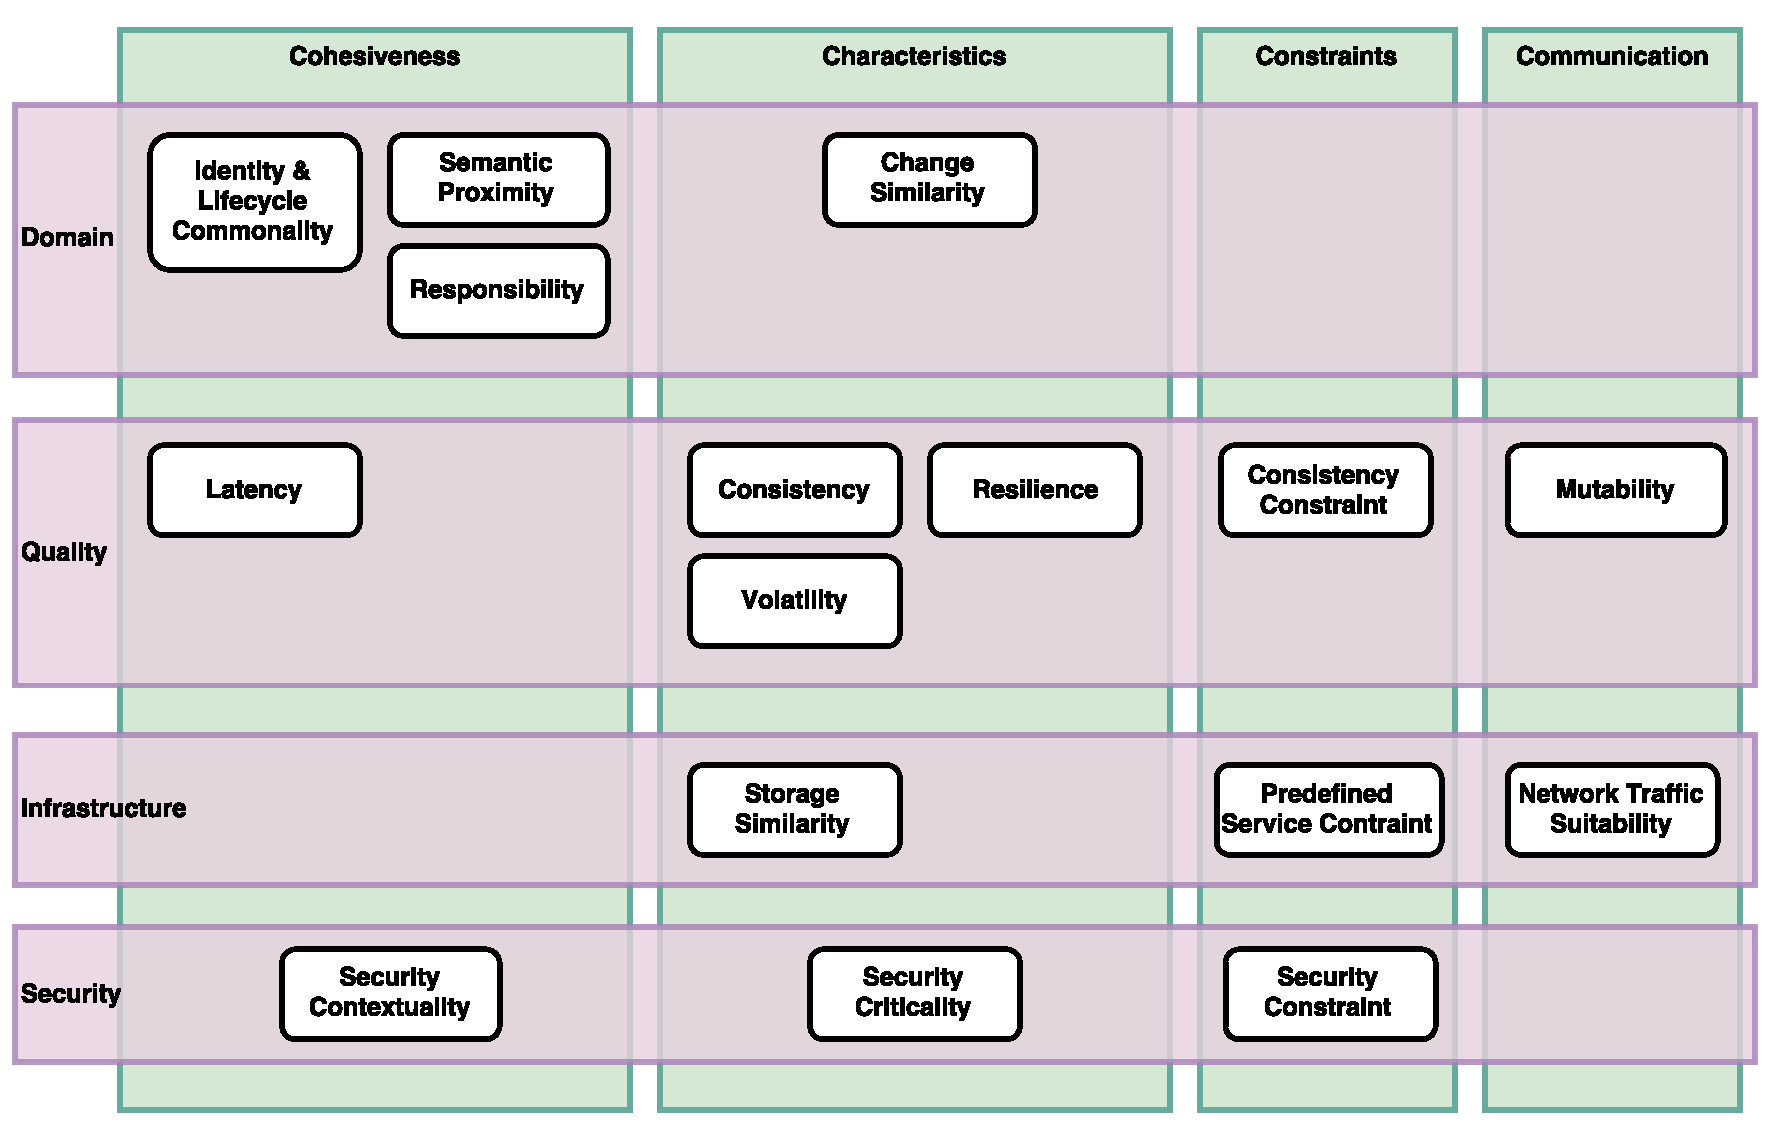
\includegraphics[scale=0.5]{diagrams/CouplingCatalog.pdf}}
	\caption{Coupling Criteria Catalog}
	\label{fig:cc-catalog-mgmt-summary}
\end{figure}


\subsubsection{Service Cutter}

Complementary to the catalog we described an approach to process coupling criteria in a software to optimize loose coupling between services and high cohesion within services. We prototypically implemented the Service Cutter, shown in Figure \ref{fig:ServiceCutter-mgmt-summary}, to verify this approach.

The Service Cutter analyzes a user's \gls{system} based on its nanoentities. Nanoentities are elements used by a service to provide business capabilities. They are defined either as data fields, operations or artifacts. 

The System is decomposed into services by defining a certain number of services and assigning all nanoentities to exactly one service.

A user can specify his system by means of well established software artifacts such as the entity-relationship model or use cases. Based on these specifications, the coupling between nanoentities is quantified with a score for each coupling criterion. 

\begin{figure}[H]
	\centering{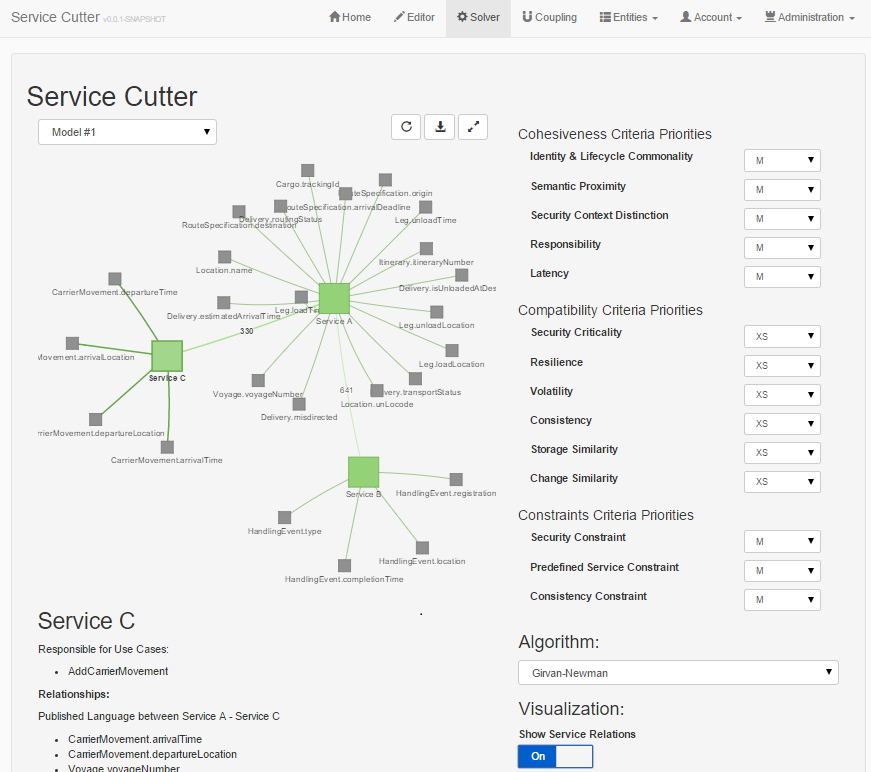
\includegraphics[scale=0.45]{images/ServiceCutter.png}}
	\caption{Screenshot Service Cutter}
	\label{fig:ServiceCutter-mgmt-summary}
\end{figure}

The exact importance of coupling is highly dependent on the context of a software system. Consistency for example is significantly divergent in a banking environment compared to an online social network. To reflect this, we rate the coupling criteria scores using priorities.

\subsubsection{Decomposition by Graph Clustering}

All scores are collected and utilized to construct a weighted undirected graph. The vertices represent nanoentities and the weighted edges embody the strength of the coupling between two nanoentities.	

Once the graph is constructed, a graph clustering algorithm calculates clusters cutting as few edges as possible. A cluster represents a candidate service. Edges connecting nodes of two clusters represent coupling between the services. This process produces candidate service cuts with high cohesion and low coupling. Figure \ref{fig:mgmt-summary-graph} illustrates a graph created to analyze a sample application.

\begin{minipage}[t]{0.6\textwidth}
	\setlength{\parskip}{5pt plus 0.1pt}
We utilized two complementary graph clustering algorithms. Girvan-Newman takes the desired number of clusters as parameter and is especially suitable for scenarios where a monolithic system is sequentially decomposed into services. The \enquote{Epidemic Label Propagation} algorithm by Leung computes the number of clusters by itself and therefore suggests a suitable number of services to the user. 

We performed tests based on an imaginary \enquote{Trading System}, heavily inspired by real banking software, and the sample application \enquote{Cargo Tracking} as introduced by Eric Evans in his book on Domain Driven Design. The Leung algorithm provided expected or applicable service cuts for both systems while Girvan-Newman only met our expectations for the Trading System. 
\end{minipage}
\begin{minipage}[t]{0.4\textwidth}	
	\begin{figure}[H]
		\begin{center}
			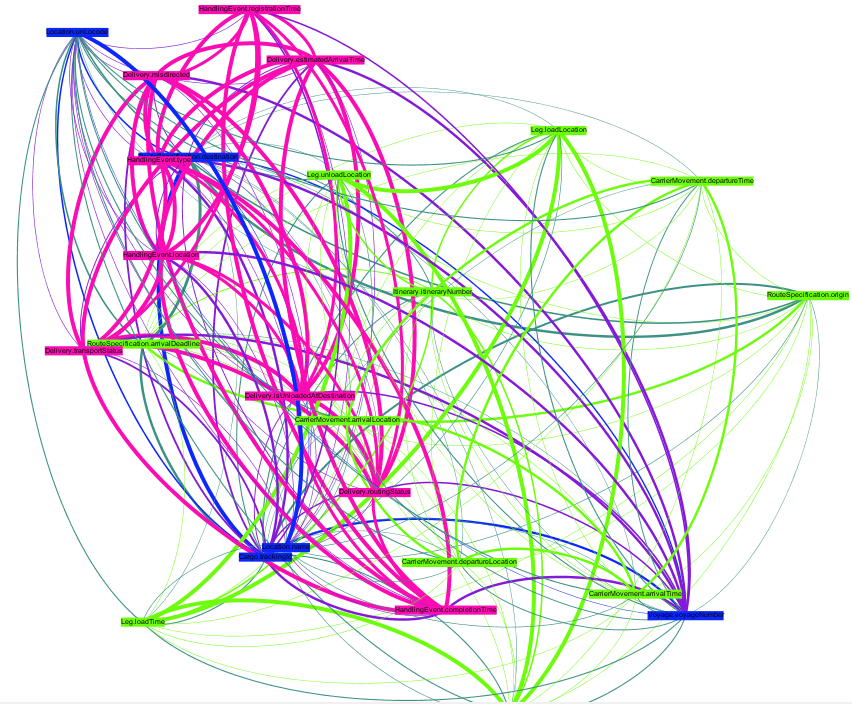
\includegraphics[scale=0.3]{images/ddd_semantic_proximity_debug.png}
			\caption{A graph created for the Cargo Tracking application. The colors represent the detected clusters.}
			\label{fig:mgmt-summary-graph}
		\end{center}
	\end{figure}
\end{minipage}

\subsubsection{Conclusion}
%TODO: könnte noch etwas knackiger sein
In our thesis, we structured the architecturally significant requirements for service decomposition into the coupling criteria catalog. The test results suggest that these criteria are quantifiable and can be optimized leveraging algorithms and software. 

The Service Cutter structures and assists the decision making process for new or already existing systems. We suggest that future projects either focus on tool development to integrate the Service Cutter into existing software development processes or invest in further research on the  scoring and the algorithms. 
